\documentclass{article}
\usepackage{amsmath, sfmath, multicol, pgfplots}
\pgfplotsset{compat = newest}
\renewcommand{\familydefault}{\sfdefault}
\pagestyle{empty}
\setlength\parindent{0pt}
\everymath{\displaystyle}
\usepackage[margin = 0.5in]{geometry}
\newcounter{pset}
\begin{document}

\subsection*{Limits P-Set}

Use a table with \emph{at least} 2 values less than and 2 vales greater than the value given in the limit to evaluate each of the following.
\begin{multicols}{3}
\begin{enumerate}
    \item $\lim_{x \to 1} (4x + 3)$
    \item $\lim_{x \to 5} (x^2-3x)$
    \item $\lim_{x \to -4} \left(\frac{1}{x+3}\right)$
\end{enumerate} \setcounter{pset}{\value{enumi}}
\end{multicols}
\smallskip
\begin{multicols}{3}
\begin{enumerate}   \setcounter{enumi}{\value{pset}}
    \item $\lim_{x \to 2} \left(\frac{x-2}{x^2-4}\right)$
    \item $\lim_{x \to -5} \left(\frac{x^2-25}{x+5}\right)$
    \item $\lim_{x \to -3}  \left(\frac{x^2+5x+6}{x^2-x-12}\right)$
\end{enumerate} \setcounter{pset}{\value{enumi}}
\end{multicols}
\bigskip 

Given the graph of $f(x)$ below, find each.
\begin{center}
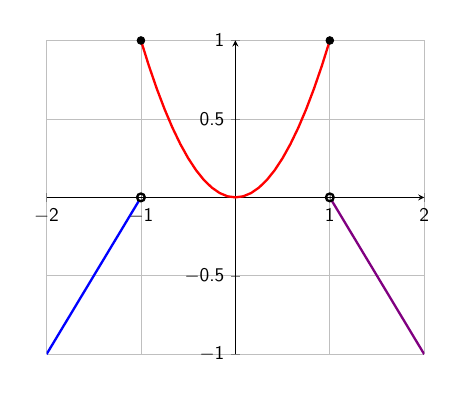
\begin{tikzpicture}[scale=0.7]
\begin{axis}
[axis lines = middle, xmin = -2, xmax = 2, xtick distance = 1, grid]
\addplot [blue, very thick, domain=-2:-1, shorten >= 2pt] {x+1};
\addplot [red, very thick, domain=-1:1] {x^2};
\addplot [violet, very thick, domain=1:2, shorten <= 2pt] {1-x};
\addplot [mark = *, only marks] coordinates {(-1,1) (1,1)};
\addplot [mark = o, only marks, very thick] coordinates {(-1,0) (1,0)};
\end{axis}
\end{tikzpicture}
\end{center}
\begin{multicols}{4}
\begin{enumerate}   \setcounter{enumi}{\value{pset}}
    \item $\lim_{x \to -1^-} f(x)$
    \item $\lim_{x \to -1^+} f(x)$
    \item $\lim_{x \to -1} f(x)$
    \item $f(-1)$
\end{enumerate} \setcounter{pset}{\value{enumi}}
\end{multicols}
\smallskip 
\begin{multicols}{4}
\begin{enumerate}   \setcounter{enumi}{\value{pset}}
    \item $\lim_{x \to 1^-} f(x)$
    \item $\lim_{x \to 1^+} f(x)$
    \item $\lim_{x \to 1} f(x)$
    \item $f(1)$
\end{enumerate} \setcounter{pset}{\value{enumi}}
\end{multicols}
\bigskip 

Find each limit algebraically.
\begin{multicols}{3}
\begin{enumerate}   \setcounter{enumi}{\value{pset}}
    % \item $\lim_{x \to 2}(2x^3 + 1)$
    \item $\lim_{x \to -1}(3x^2 + 6x)$
    \item $\lim_{x \to 0}\sqrt{5x + 49}$
    \item $\lim_{x \to 0}\left(\frac{x^2-4}{x^2+4}\right)$
\end{enumerate}     \setcounter{pset}{\value{enumi}}
\end{multicols}
\smallskip
\begin{multicols}{3}
\begin{enumerate}   \setcounter{enumi}{\value{pset}}
    \item $\lim_{x \to -3}\left(\frac{x^2-x-12}{x+3}\right)$
    \item $\lim_{x \to 1}\left(\frac{x^2-1}{x-1}\right)$
    \item $\lim_{x \to -3}\left(\frac{x^2+x-6}{x^2+2x-3}\right)$
\end{enumerate}     \setcounter{pset}{\value{enumi}}
\end{multicols}
\bigskip

For $f(x) = 2x^2$, evaluate each.
\begin{multicols}{2}
\begin{enumerate}   \setcounter{enumi}{\value{pset}}
    \item $\lim_{h \to 0} \frac{f(1+h)-f(1)}{h}$
    \item $\lim_{h \to 0} \frac{f(3+h)-f(3)}{h}$
\end{enumerate}
\end{multicols}

\newpage

\texttt{Key}

\begin{enumerate}
    \item 7
    \item 10
    \item $-1$
    \item $\frac{1}{4}$
    \item $-10$
    \item $\frac{1}{7}$
    \item 0
    \item 1
    \item Does not exist
    \item 1
    \item 1
    \item 0
    \item Does not exist
    \item 1
    \item $-3$
    \item 7
    \item $-1$
    \item $-7$
    \item 2
    \item $\frac{5}{4}$
    \item 4
    \item 12
\end{enumerate}

\end{document}
